% Transactions in big-data platforms
In recent years, transaction processing~\cite{Gray:1992:TPC:573304} technologies have paved their way into multi-petabyte big data 
platforms~\cite{Percolator2010,Spanner2012,Omid2017}. 
%In some cases, they are built into the storage system itself~\cite{Spanner2012} whereas in the others they are standalone services~\cite{Omid2017}. 
Modern industrial transaction processing systems~\cite{Percolator2010, Omid2017, tephra, cockroach} complement 
existing underlying NoSQL key-value storage with {\em atomicity}, {\em consistency}, {\em isolation\/} and {\em durability} (ACID) 
semantics that enable programmers to perform complex data manipulation without over-complicating their applications. 
Google's Percolator~\cite{Percolator2010} pioneered a transaction processing API atop the Bigtable storage. Apache 
Tephra and Omid followed suit with Apache HBase~\cite{hbase}. 

Transaction support in huge-scale applications was initially motivated by specific use cases like real-time content indexing for 
web search~\cite{Percolator2010, Omid2017} but  rapidly evolved into a wealth of OLTP and operational analytics 
applications (e.g.,~\cite{Borthakur:2011, F1-2013}). In recent years, we see data management platforms provide ACID transactions as part of a full-fledged 
SQL interface, e.g., Google Spanner~\cite{Spanner2012}, Apache Phoenix~\cite{phoenix}, and CockroachDB~\cite{cockroach}. 
%This allows for  reuse, and affords them the flexibility to continue to offer capabilities from the NoSQL world alongside new functionalities. 

Similarly to many technologies, the adoption of transactions took a  ``functionality-first" trajectory. 
For example, the developers of Spanner~\cite{Spanner2012} wrote:
\begin{quote}
  ``We believe it
is better to have application programmers deal with performance problems due to overuse 
of transactions as bottlenecks arise, rather than always coding around the lack of transactions''. 
\end{quote}
Yet the expectation for high performance is rapidly picking up. 
Whereas early transaction systems were  latency-insensitive~\cite{Percolator2010, Omid2017}, 
with the thrust into new interactive domains like 
social networks~\cite{chatter},  %logging~\cite{},
messaging~\cite{Borthakur:2011} and algorithmic trading~\cite{opentsdb} 
latency becomes essential;   
SLAs for interactive user experience
mandate that simple updates and point queries  complete within single-digit milliseconds. 
This paper is motivated by such  applications.

\remove{ % Idit: removed the following two paragraphs for blind review; moved some content above and below
Consider, for example, the platform powering Yahoo! Mail, which serves hundreds of millions of users. 
The Mail backend ingests billions of messages daily; messages undergo both machine 
classification (e.g., for spam filtering, thread detection, and ``smart views''~\cite{smart-view}),
%\footnote{\footnotesize{\url{https://yahoohelpcommunity.tumblr.com/post/118485031125/getting-to-know-smart-views-in-yahoo-mail}}}
and user manipulation (e.g., starring, tagging, and moving between folders).    
Mail users browse their mail and search for content, issuing many billions of requests a day; they
expect a consistent experience -- e.g., messages  do not 
disappear when moved between folders, starred content gets prioritized in search, folder counters are reliable, etc.

The Yahoo! Mail metadata platform is built on top of Apache HBase~\cite{hbase}, 
which provides reliable and scalable key-value storage. The system's first generation
was built without transaction support. This exposed  developers to very complex programming scenarios 
to achieve ACID behavior (e.g., consistent folder listings, atomic updates of multiple counters). 
%We would like to build the next generation of the system using a transaction API on top of HBase.
We have looked into building the next generation using  Omid~\cite{omid}, 
an Apache Incubator project which provides a transaction API on top of HBase, and 
is already in use at large scale at Yahoo~\cite{Omid2017}.
Unfortunately, while this makes programming much easier, it also jeopardizes 
the real-time latency SLA for interactive user experience. For example,  
simple updates and point queries must complete within single-digit milliseconds.
whereas Omid, which was designed for throughput-oriented data pipelines~\cite{Omid2017}, 
can induce latencies of tens to hundreds of milliseconds under high loads. 

Motivated by this example, 
}%remove

% Drum roll 

Our main contribution is supporting low-latency {\em and\/} high-throughput transaction processing  for HBase 
\inred{via a solution that is appropriate  for multi-tenancy scenarios}.  
We further extend Omid's API with functionality required by
a SQL engine running atop it.
Similarly to other modern transaction managers~\cite{Percolator2010,Spanner2012,Omid2017,tephra,cockroach},
we provide a (somewhat relaxed) variant of \emph{snapshot isolation (SI)}~\cite{DBLP:conf/sigmod/BerensonBGMOO95},
which scales better than traditional serializability implementations; the service's API and semantics are defined in  Section~\ref{sec:api}.  

Our prototype is based on Apache Incubator Omid~\cite{omid}, but dissipates the principal bottleneck present therein.
%in the prior implementations the overhead of begin and commit operations. 
Its advantage is maximized for short  transactions, which are prevalent in latency-sensitive applications.
Our system processes  such transactions in a handful of milliseconds, whereas Omid, 
which was designed for throughput-oriented data pipelines~\cite{Omid2017}, 
can induce latencies of tens to hundreds of milliseconds under high loads. 
The new protocol also doubles the system throughput.
%Moreover, it is amenable to a simpler high availability solution than the original design. 
%, which is \inred{an order of magnitude higher than} previously achievable limits. 
%Different aspects of our protocol are inspired by other systems, while their combination is novel.
%, to the best of our knowledge. 

The performance  improvement  is achieved in two steps, as depicted in Figure~\ref{fig:evolution}.  
%by two design changes.
First, in Section~\ref{sec:ll}, we create a new low latency version of Omid, \sysll. It  
distributes persistent writes of transaction commit records, which is a centralized bottleneck in Omid. 
\sysll\ uses Omid's centralized transaction manager for timestamp allocation and conflict detection, 
but relieves it of performing I/O. 
It is important to  note that we distribute the writes of commit records, but not the records themselves.
\inred{
This is in contrast to Percolator, which distributed the actual commit records in database tables, 
under the assumption  that all transactions have permission 
to access all tables, which is common in single-application settings, but is often not the case 
in multi-tenancy scenarios.
}
We further explore the design space of transaction processing protocols (in Section~\ref{sec:ll}), 
and implement a variant of Omid that uses Percolator's \emph{two-phase commit (2PC)} approach to 
conflict detection~\cite{Percolator2010}, which we call \syspc. 

  
Second, in Section~\ref{sec:alg} we introduce a novel \emph{fast path} algorithm for short single-key transactions, which 
executes short transactions without the begin/commit overhead, 
 almost as fast as native HBase operations. This entails minor extensions to the underlying 
data store. We call the resulting system \sys. Note that
the fast path is orthogonal to other protocol aspects, and can be supported in other 
transaction processing services. 
%, to enable local commits directly within the storage layer and verify the correctness of general 
%transactions in presence of such commits. 

\begin{figure}
  \centerline{
        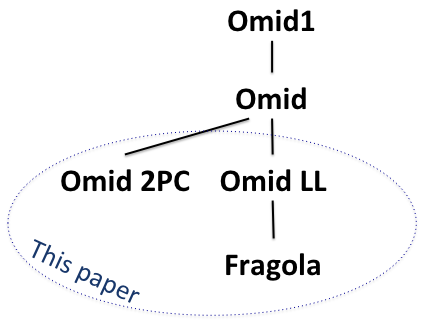
\includegraphics[width=0.75\columnwidth]{figs/OmidEvolution}	
  }
\caption{The evolution of Omid. We develop a low latency version Omid-LL, and extend it to support fast-path transactions in \sys.
              We implement a variant based on two phase commit, \syspc, for comparison.}
\label{fig:evolution}
\end{figure}


%We have implemented {\sys\/} %\footnote{\url{https://github.com/yonigottesman/incubator-omid/tree/localTransactions}} 
Our implementations are 
based on the open source Omid code\footnote{\url{https://omid.incubator.apache.org}}.
To support \syspc\ and \sys, we further extended  HBase  to enable locking and the fast path, resp. 
%\footnote{\url{https://github.com/yonigottesman/hbase_local_transactions/tree/0.98-add-rmw}}. 
Our code is publicly available on github\footnote{\small{Omitted for blind review.}}
and since \sysll\ does not require HBase extensions.
\inred{We hope to contribute it back to the Omid open-source project.}
%and we are currently productionalizing \sysll, (which does not require HBase extensions),  
%and contributing the changes back to the Omid open-source project.
 
 \inred{Describe the functionality extensions for SQL and refer to the new section that will present them.}
 
 Section~\ref{sec:eval} presents our experiments on mid-range hardware, which show substantial performance improvements.
Under low load, \sysll\ transactions are 4x to 5x faster than Omid's, 
and \sys\ further reduces the latency of short transactions by another $55\%$ on average.
As system load increases, Omid's latency surges (at  $\sim\!\!\!150$K tps in our tests),  
whereas \sys's remains stable. \syspc\ performs similarly to \sysll, except on long transactions
where it is slower; e.g., on $10$-key transactions \syspc\ is $30\%$ slower than \sysll.
% until we generate a higher load ($\sim\!\!500$K tps)
%, and increases four-fold at 500K tps.  
Fast path transactions incur no scalability
bottlenecks, and execute at the low latency of native HBase operations regardless of system load
(thanks to HBase's near perfect horizontal scalability).
This comes at the cost of a minor (15-25\%) negative impact on longer transactions. 
%{\inred{The system scales beyond 1M transactions per second on medium-end hardware,
%which surpasses Omid at least 4x.}} 
Additionally, \sys\ has negligible impact on  transaction abort rates.

\remove{
% \Idit{The roadmap below is not essential; maybe replace with summary of contributions.}
%The remainder of this paper is organized as follows:
In Section~\ref{sec:api} we define the  API and semantics of a transaction processing service. 
Section~\ref{sec:ll} describes \sysll, and 
%Section~\ref{sec:ha} discusses its high availability mechanism. 
Section~\ref{sec:alg} presents \sys.  Our evaluation is reported in 
Section~\ref{sec:eval}.
%In Section~\ref{sec:context} we generalize the fast path algorithm, and explain how it could be implemented in other systems. 
}

We review related work in Section~\ref{sec:related} and conclude with Section~\ref{sec:conclusions}.
In summary, our contributions are as follows:
\begin{enumerate}
    \setlength{\itemsep}{1pt}
    \setlength{\parskip}{1pt}
    \setlength{\parsep}{1pt}  
\item We implement \sysll, a low-latency distributed transaction engine \inred{amenable to multi-tenancy}; 
we plan to contribute it  to the Apache Omid project.
%which improves latency by 5x and doubles throughput; 
%we are working to incorporate in  production;
\item We explore the design space of transaction processing engines for NoSQL data stores, 
highlighting the tradeoffs between various design choices.  
\item We design a novel fast path for short transactions and implement it in \sys.
\item We extend Omid with functionality that facilitates implementing a SQL API. 
\item We extensively evaluate the systems.
\end{enumerate}